\chapter{Mô hình đề xuất}
\section{Hình ảnh}
\begin{figure}[H]
	\centering
	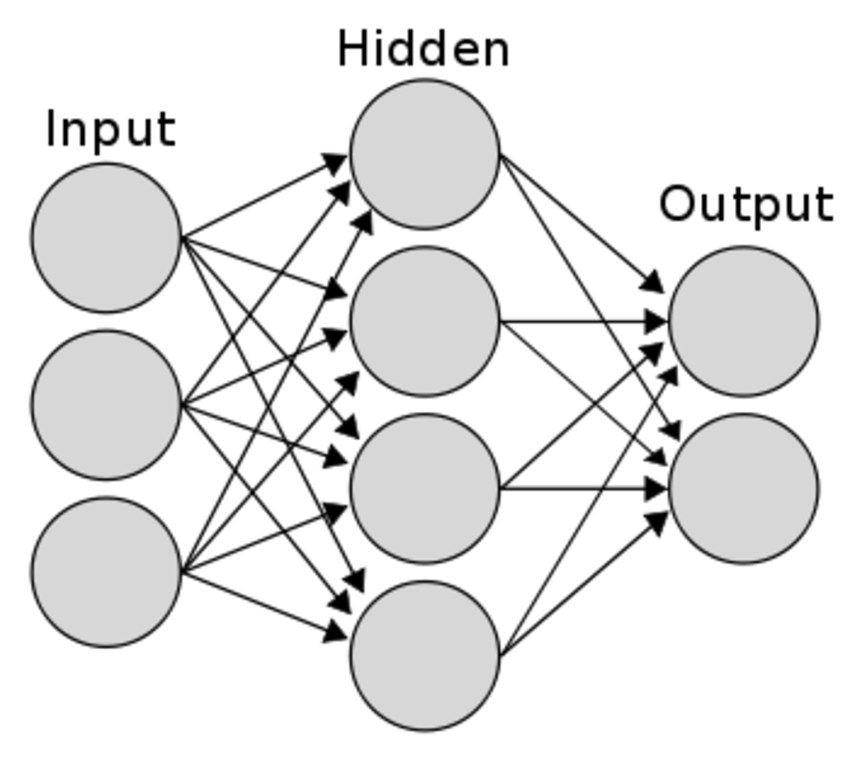
\includegraphics[width=0.4\textwidth]{picture/pic3}
	\caption{Mạng noron nhân tạo}
\end{figure}

\begin{figure}[H]
	\centering
	\begin{subfigure}{0.45\textwidth}
		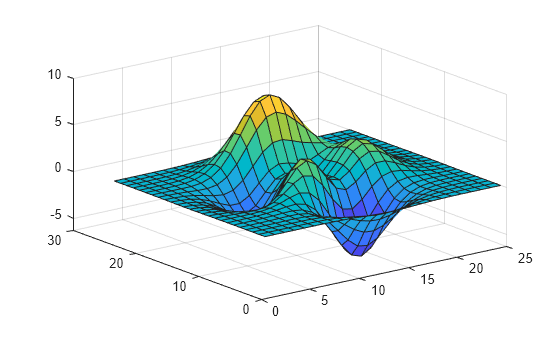
\includegraphics[width=1\textwidth]{picture/pic1}
		\caption{3D}
	\end{subfigure}
	\begin{subfigure}{0.45\textwidth}
		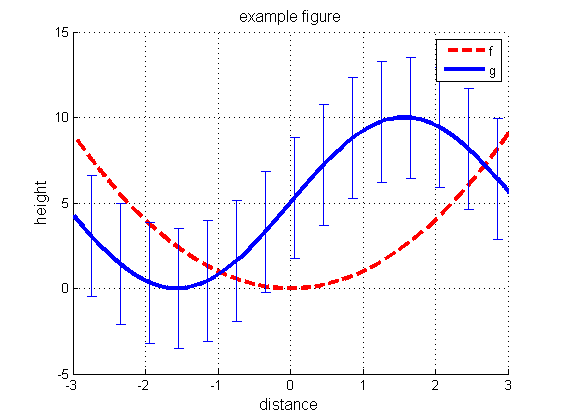
\includegraphics[width=1\textwidth]{picture/pic2}
		\caption{2D}
	\end{subfigure}
	\caption{Đồ thị}
\end{figure}
\section{Bảng biểu}
\begin{table}[H]
	\centering
	\caption{Bảng giá trị của đồ thị hàm số $y=x+1$}
	\begin{tabular}{|c|c|c|c|c|}
		\hline
		$x$& 0 & 1& 2 & 3\\
		\hline
		$y$&1 & 2& 4 &5\\
		\hline
	\end{tabular}
\end{table}

\begin{equation}
f(x) = \frac{a_0}{2} + \sum_{n=1}^{\infty} \left( a_n \cos\left(\frac{2\pi n x}{T}\right) + b_n \sin\left(\frac{2\pi n x}{T}\right) \right)
\label{eq:chuoi_fourier}
\end{equation}